\documentclass{article}

\usepackage[square,numbers]{natbib}
\bibliographystyle{unsrtnat}

\usepackage{hyperref}

\usepackage{tikz}
\usetikzlibrary{chains,matrix,graphs,scopes,decorations.shapes,arrows,shapes}
\tikzset{
  nonterminal/.style={
    % The shape:
    rectangle,
    % The size:
    minimum size=6mm,
    % The border:
    very thick,
    draw=red!50!black!50,
    % The filling:
    top color=white,
    bottom color=red!50!black!20,
  },
  terminal/.style={
    % The shape:
    rounded rectangle,
    minimum size=6mm,
    % The rest
    very thick,draw=black!50,
    top color=white,bottom color=black!20,
    font=\ttfamily},
  instruction/.style={
    % The shape:
    rectangle,
    minimum size=6mm,
    % The rest
    draw=white,
    top color=white,bottom color=white},
  skip loop/.style={to path={-- ++(0,#1) -| (\tikztotarget)}}
}
{
  \tikzset{terminal/.append style={text height=1.5ex,text depth=.25ex}}
  \tikzset{nonterminal/.append style={text height=1.5ex,text depth=.25ex}}
  \tikzset{instruction/.append style={text height=1.5ex,text depth=.25ex}}
}

\listfiles

\title{T7 compiler manual}
\author{Nicolas Mauger}
\date{\today}

\begin{document}
    \maketitle

    \newpage

    \begin{abstract}
	    T7 is a project started in August 2018 originally written by Nicolas Mauger.
	    It's a step-by-step approach to compiler development mostly based on the books
	    \textit{Compiler Design In C \cite{CompilerDesignInC}} and \textit{Systematic Software
	    Development Using VDM \cite{VDMdevelopment}}. \\
	    All documents in this project are subject to the CeCILL license. You should have receive a
	    copy of the CeCILL free software license agreement version 2.1 along with this program and
	    documents; if not, please visit
	    \href{http://www.cecill.info/licences/Licence_CeCILL_V2.1-en.txt}{www.cecill.info} or send
	    an email at \href{mailto:nicolas@mauger.cafe}{nicolas@mauger.cafe}.
    \end{abstract}

    \tableofcontents

        \section{Basic concepts and naive implementation}
        Our very first compiler is split in three parts : a lexical analyzer (see \texttt{lex.*}
        files), a parser (see \texttt{parse.*} files) and a code generator.

            \subsection{Short lexical analyzer}
            The lexical analyzer will simply \textit{tokenize} all the sources and translates all
            the lexemes\footnote{A lexeme is a sequence of characters in the source program that
            matches the pattern for a token and is identified by the lexical analyzer as an instance
            of that token.} into a simple computable representation. Their representations will be
            easier to parse.

            \subsection{Our very first parser}
            We start by parsing simple arithmetical operation. First we decompose statements in four
            simple syntax who can be found in any basic programmation langague who accept
            arethmetical operation. Moreover, expressions, terms and actors can be used recursively:
            expression contains terms which contain factors which contain expressions...etc. At this
            step we can already catch error if the operation does not respect theirs following
            syntax schemes.

            \begin{figure}[!ht] % Statment syntax
            \label{fig:statmentSyntax}
            \centering
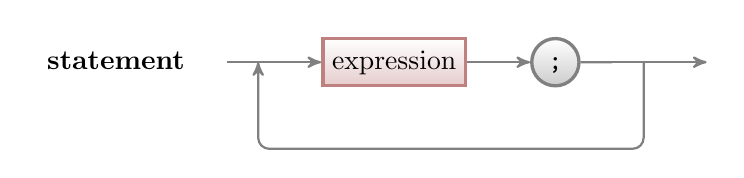
\begin{tikzpicture}[point/.style={coordinate},>=stealth',thick,draw=black!50,
                    tip/.style={->,shorten >=0.007pt},every join/.style={rounded corners},
                    hv path/.style={to path={-| (\tikztotarget)}},
                    vh path/.style={to path={|- (\tikztotarget)}},
                    text height=1.5ex,text depth=.25ex]
  \matrix[ampersand replacement=\&,column sep=4mm] {
    \node (statment) [instruction] {\textbf{statement}};                    \&
    \node (p1)  [point]  {}; \&  \node (p1a)   [point]       {};           \&
    \node (p2)  [point]  {}; \&  \node (expr1) [nonterminal] {expression}; \&
    \node (p3)  [point]  {}; \&  \node (dot)   [terminal]    {;};          \&
    \node (p4)  [point]  {}; \&  \node (p4a)   [point]       {};           \&
    \node (p5)  [point]  {}; \&  \node (p5a)   [point]       {};           \\
  };

  { [start chain]
    \chainin (statment)[];
    \chainin (p1);
    \chainin (p1a)    [join,join=with p4a by {skip loop=-11mm,tip}];
    \chainin (p2)     [join];
    \chainin (expr1)  [join=by tip];
    \chainin (p3)     [join];
    \chainin (dot)    [join=by tip];
    \chainin (p4)     [join];
    \chainin (p4a)    [join];
    \chainin (p5)     [join];
    \chainin (p5a)    [join=by tip];
  }
\end{tikzpicture}
            \end{figure}

            \begin{figure}[!ht] % Expression syntax
            \label{fig:expressionSyntax}
            \centering
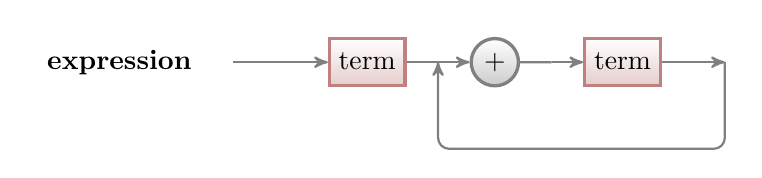
\begin{tikzpicture}[point/.style={coordinate},>=stealth',thick,draw=black!50,
                    tip/.style={->,shorten >=0.007pt},every join/.style={rounded corners},
                    hv path/.style={to path={-| (\tikztotarget)}},
                    vh path/.style={to path={|- (\tikztotarget)}},
                    text height=1.5ex,text depth=.25ex]
  \matrix[ampersand replacement=\&,column sep=4mm] {
    \node (expression) [instruction] {\textbf{expression}};         \&
    \node (p1)  [point]  {}; \&  \node (p1a)  [point]       {};     \&
    \node (p2)  [point]  {}; \&  \node (term1)[nonterminal] {term}; \&
    \node (p3)  [point]  {}; \&  \node (plus) [terminal]    {$+$};  \&
    \node (p4)  [point]  {}; \&  \node (term2)[nonterminal] {term}; \&
    \node (p5)  [point]  {}; \&  \node (p5a)  [point]       {};     \\
  };

  { [start chain]
    \chainin (expression)[];
    \chainin (p1);
    \chainin (p1a)    [join];
    \chainin (p2)     [join];
    \chainin (term1)  [join=by tip];
    \chainin (p3)     [join,join=with p5a by {skip loop=-11mm,tip}];
    \chainin (plus)   [join=by tip];
    \chainin (p4)     [join];
    \chainin (term2)  [join=by tip];
    \chainin (p5)     [join];
    \chainin (p5a)    [join=by tip];
  }
\end{tikzpicture}
            \end{figure}
            \begin{figure}[!ht] % Term syntax
            \label{fig:TermSyntax}
            \centering
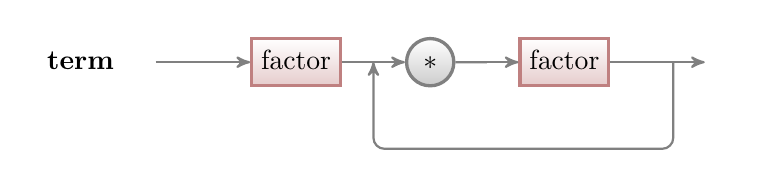
\begin{tikzpicture}[point/.style={coordinate},>=stealth',thick,draw=black!50,
                    tip/.style={->,shorten >=0.007pt},every join/.style={rounded corners},
                    hv path/.style={to path={-| (\tikztotarget)}},
                    vh path/.style={to path={|- (\tikztotarget)}},
                    text height=1.5ex,text depth=.25ex]
  \matrix[ampersand replacement=\&,column sep=4mm] {
    \node (expression) [instruction] {\textbf{term}};                \&
    \node (p1)  [point]  {}; \&  \node (p1a)  [point]       {};           \&
    \node (p2)  [point]  {}; \&  \node (factor1)[nonterminal] {factor}; \&
    \node (p3)  [point]  {}; \&  \node (times) [terminal]    {$*$};          \&
    \node (p4)  [point]  {}; \&  \node (factor2)[nonterminal] {factor}; \&
    \node (p5)  [point]  {}; \&  \node (p5a)  [point]       {};           \&
    \node (p6)  [point]  {}; \&  \node (p6a)  [point]       {};           \\
  };

  { [start chain]
    \chainin (expression)[];
    \chainin (p1);
    \chainin (p1a)     [join];
    \chainin (p2)      [join];
    \chainin (factor1) [join=by tip];
    \chainin (p3)      [join,join=with p5a by {skip loop=-11mm,tip}];
    \chainin (times)   [join=by tip];
    \chainin (p4)      [join];
    \chainin (factor2) [join=by tip];
    \chainin (p5)      [join];
    \chainin (p5a)     [join];
    \chainin (p6)      [join=by tip];
  }
\end{tikzpicture}
            \end{figure}
            \begin{figure}[!ht] % Factor syntax
            \label{fig:FactorSyntax}
            \centering
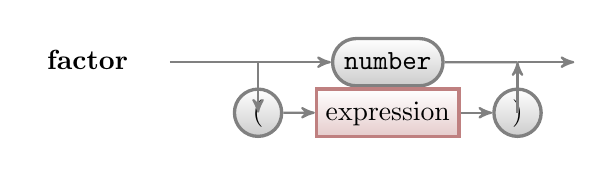
\begin{tikzpicture}[point/.style={coordinate},>=stealth',thick,draw=black!50,
                    tip/.style={->,shorten >=0.01pt},every join/.style={rounded corners},
                    hv path/.style={to path={-| (\tikztotarget)}},
                    vh path/.style={to path={|- (\tikztotarget)}},
                    text height=1.5ex,text depth=.25ex]

  \matrix[ampersand replacement=\&,column sep=4mm] {
    % First row:
    \node (factor) [instruction] {\textbf{factor}};                  \&
    \node (p1)  [point]  {}; \&  \node (p1a)    [point]    {};       \&
    \node (p2)  [point]  {}; \&  \node (number) [terminal] {number}; \&
    \node (p3)  [point]  {}; \&  \node (p3a)    [point]    {};       \\
    % Second row:
    \& \& \& \node (LP)  [terminal]{$($}; \&
    \node (ex) [nonterminal]{expression}; \& \node (RP) [terminal]{$)$}; \\
  };

  { [start chain]
    \chainin (factor)[];
    \chainin (p1)      ;
    \chainin (p1a)   [join];
    \chainin (p2)    [join];
    { [start branch=ex]
        \chainin (LP) [join=by {vh path,tip}];
        \chainin (ex) [join=by tip];
        \chainin (RP) [join=by tip];
        \chainin (p3) [join=by {hv path,tip}];
    }
    \chainin (number)[join=by tip];
    \chainin (p3)    [join];
    \chainin (p3a)   [join=by tip];
  }

\end{tikzpicture}
            \end{figure}

            \subsection{The code generator}
            The parse tree created in the previous step can be simply used by a different program to
            generate code. But most of the modern compiler, the code generation is a part of parse
            process. Indeed, the parse tree created can be used to create an intermediate language,
            like a super-assembly, to perform specific tasks like optimisation, compression and
            platform specific binary generation. This is this intermediate language method how will
            be used in T7.

\bibliography{main}
\end{document}
